\documentclass[12pt,a4paper]{article}
\usepackage{cmap}
\usepackage[utf8]{inputenc}
\usepackage[T1,T2A]{fontenc}
\usepackage[english,russian]{babel}
\usepackage{booktabs,array,graphicx}
\usepackage{caption,float,qrcode}
\usepackage{geometry,hyperref,indentfirst}
\geometry{margin=25mm}
\hypersetup{unicode=true,colorlinks=true,urlcolor=blue,linkcolor=black}
\setlength{\parindent}{1.25cm}
\setlength{\parskip}{0pt}
\setlength{\emergencystretch}{2em}
\DeclareCaptionLabelSeparator{emdash}{\space---\space}
\captionsetup[figure]{justification=centering,singlelinecheck=false,labelsep=emdash}
\addto\captionsrussian{\renewcommand{\figurename}{Рис.}}
\linespread{0.96}
\begin{document}
\hypersetup{pageanchor=false}
\begin{titlepage}
\begin{center}
{\large МОСКОВСКИЙ АВИАЦИОННЫЙ ИНСТИТУТ\\
(НАЦИОНАЛЬНЫЙ ИССЛЕДОВАТЕЛЬСКИЙ УНИВЕРСИТЕТ)}
\vspace{18pt}
{\large Факультет информационных технологий и прикладной математики}

{\large Кафедра вычислительной математики и~программирования}
\vfill
{\large\textbf{Лабораторная работа №14 по курсу\\ «Информационный поиск»}}
\vspace{12mm}

{\large\textbf{Построение сниппетов поисковой выдачи}}
\vfill
\begin{flushright}
\begin{tabular}{@{}r@{:\hspace{0.6em}}l@{}}
\textit{Студент} & К.\,А. Арусланов\\
\textit{Группа} & М8О-403Б-23\\
\textit{Преподаватель} & А.\,А. Кухтичев\\
\textit{Дата} & 08.11.2026\\
\textit{Оценка} &
\end{tabular}
\end{flushright}
\vfill
Москва, 2026
\end{center}
\end{titlepage}
\hypersetup{pageanchor=true}
\setcounter{page}{2}
\tableofcontents
\newpage

\section{Постановка задачи}
Для найденных документов построить короткие фрагменты исходного текста,
объясняющие совпадение с запросом. Показывать сниппеты в командной строке
и веб-выдаче. Результаты поиска
и их порядок должны сохраняться.

\section{Метод решения}
\subsection{Доступ к исходному тексту}
Поисковый индекс ЛР7--ЛР13 хранит заголовки и координаты, но не тела
документов. Тексты находятся в неизменяемом снимке MAIIR3 из 478,833
документов. Для быстрого доступа создан отдельный файл смещений:
для каждого ID записаны положение и длина заголовка и текста.
Файл создаётся однократно потоковым проходом по снимку и занимает
19,153,352 байта; тела документов в оперативную память при построении
не загружаются. При запросе читаются только тексты показанных документов.

Файл смещений содержит версию формата, размер снимка, число документов
и контрольную сумму записей. При открытии проверяются границы и порядок ID.
Заголовок каждого показанного документа сравнивается побайтово с заголовком
из поискового индекса. Это защищает от случайной подмены снимка или
смещений. При отсутствии файла CLI может восстановить смещения при
открытии, но такой путь не подходит для частых запросов.

\subsection{Выбор фрагмента}
Исходный текст делится на предложения по точке, вопросительному и
восклицательному знакам перед пробелом, а также по переводу строки.
Токенизация использует те же правила \texttt{gaming-v3}, что и индекс.
В режиме лемм варианты терминов сопоставляются через тот же словарь.
Для предложения подсчитываются число разных слов запроса и число
совпадений. Компактное расположение совпадений повышает оценку;
при равенстве предпочтение отдаётся более раннему предложению.
Если в тексте нет слов запроса, показывается его начало.

После выбора предложения сниппет расширяется соседними предложениями
в пределах того же абзаца. Это даёт контекст коротким предложениям и
не захватывает соседние блоки рекомендаций сайта. Фрагмент ограничивается
600 байтами, по возможности вокруг первого совпадения. Обрезка выполняется
только на границе символа UTF-8.
Ответ CLI содержит сам текст, байтовые диапазоны совпадений внутри него
и признаки обрезки слева и справа. Веб-форма преобразует эти диапазоны
в подсветку \texttt{<mark>} после HTML-экранирования фрагмента.
Текст сниппета выводится меньшим, приглушённым серым шрифтом;
совпавшие слова остаются контрастными.
Код выбора и хранения смещений написан на C++ без STL-контейнеров.

\section{План тестирования}
\begin{center}
\small
\begin{tabular}{@{}p{55mm}p{88mm}@{}}
\toprule
Случай & Ожидаемый результат\\
\midrule
Несколько предложений & Выбирается лучшее, добавляются соседи из того же абзаца\\
Русский UTF-8 & Диапазоны выделяют полные слова в байтовой строке\\
Прямое чтение и файл смещений & Сниппеты и порядок результатов одинаковы\\
Повреждённый файл смещений & Ошибка контрольной суммы до выдачи документов\\
Текст отсутствует & Пустой сниппет без ошибки поиска\\
HTML в тексте документа & Теги экранированы; подсвечены только слова запроса\\
Реальный снимок и веб-форма & CLI возвращает фрагменты, HTTP-ответ содержит подсветку\\
\bottomrule
\end{tabular}
\end{center}

Шесть GoogleTest вызывают C++-поиск на синтетическом корпусе: проверяют
выбор предложения, точность UTF-8 диапазонов, совпадение двух способов
чтения, отказ на повреждении, привязку снимка к индексу, обрезку длинного
предложения и пустой текст. Три Python unittest
проверяют передачу параметров ядру и безопасное отображение HTML.
Весь набор предыдущих лабораторных также запущен на текущих исходниках.

\section{Результаты}
\subsection{Проверка на полном снимке}
Файл смещений успешно построен для 478,833 документов. Скрипт
\path{run_lab14.py} выполнил пять запросов на упакованном индексе:
TF-IDF по словоформам и леммам, а также булев поиск. Для запроса
\texttt{doom AND eternal} булев поиск нашёл 1,392 документа;
для первого результата выбран фрагмент о выпуске Doom Eternal.
Для TF-IDF запроса \texttt{doom eternal} найдено 9,170 документов;
первые пять результатов и сниппеты сохранены в
\path{lab14/examples.json}. HTTP-запрос к веб-форме вернул код 200,
на сохранённой странице \path{lab14/web_example.html} есть 27
подсвеченных вхождений.
Для запроса \texttt{"игры ps plus"} AND \texttt{сентябрь} по леммам найдено шесть
документов. У первых двух короткое предложение со словами запроса
расширилось до полного абзаца: 559 и 542 байта вместо одной строки.
У третьего документа слова встречаются только в блоке «Читайте также»;
переходить в соседний абзац здесь означало бы показывать чужой контекст.

\begin{figure}[H]
\centering
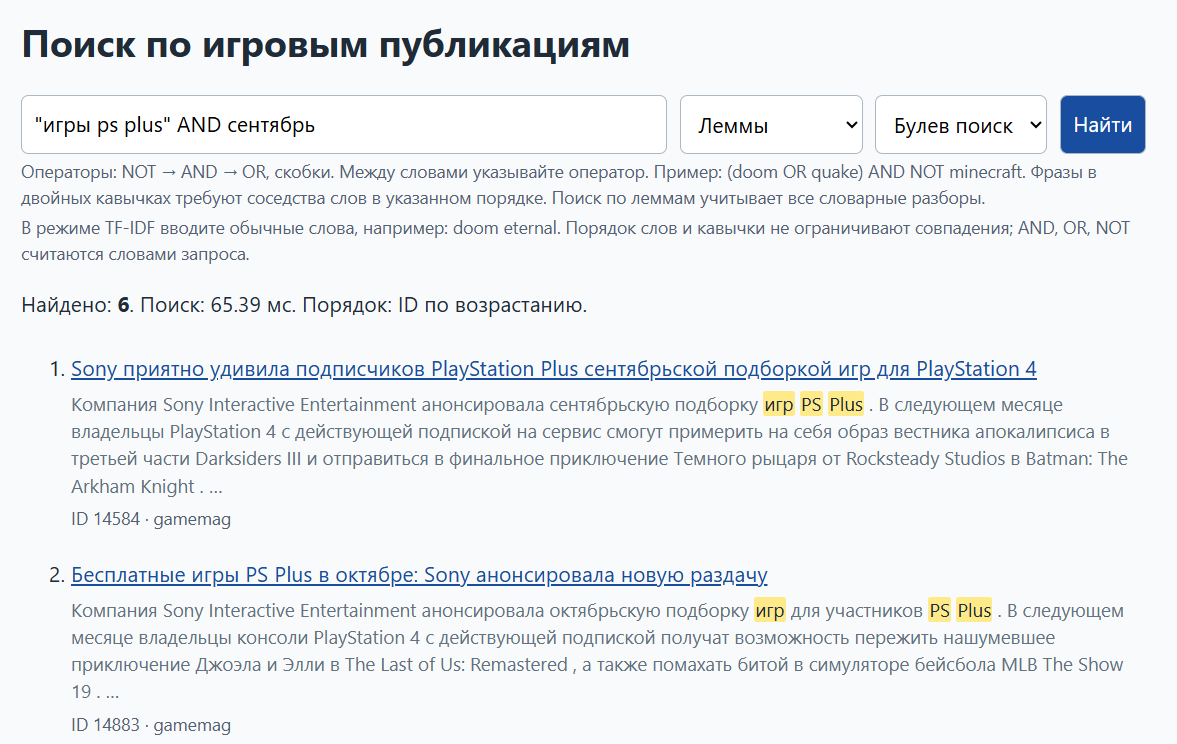
\includegraphics[width=0.98\linewidth]{img/ps_plus_september.png}
\caption{Булев поиск по леммам: запрос \texttt{"игры ps plus"} AND \texttt{сентябрь};
два первых результата с расширенными сниппетами}
\end{figure}

\begin{figure}[H]
\centering
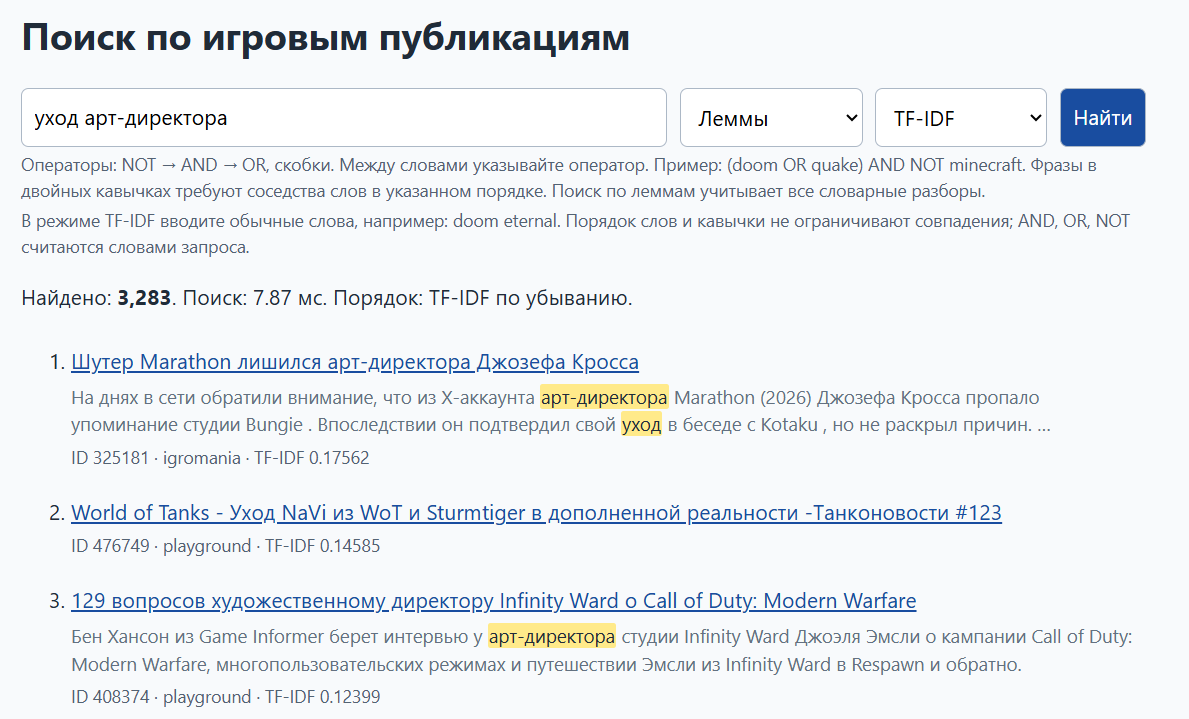
\includegraphics[width=0.98\linewidth]{img/art_director.png}
\caption{TF-IDF по леммам: запрос «уход арт-директора»; у второго
результата текст документа отсутствует, поэтому сниппет пуст}
\end{figure}
\clearpage

С файлом смещений полный вызов CLI для запроса \texttt{doom eternal}
занял 0,149 с. Первый вариант, просматривавший снимок при каждом
запросе, требовал около 9 с. Это наблюдения одного запуска при тёплом
кэше, включая открытие индекса и подготовку выдачи, а не гарантированное
время ответа на другом компьютере.

\subsection{Автотесты}
Тесты ЛР14: 6/6 GoogleTest и 3/3 Python unittest. Полный регрессионный
прогон: 153/153 CTest и 294/294 Python-тестов, без пропусков;
для интеграционных проверок запущена отдельная временная MongoDB.
Отдельные тестовые случаи и результаты записаны в
\path{lab14/full/tests.txt}; сводка находится в
\path{lab14/full/summary.json}.

Исходники, команды сборки и повторения эксперимента описаны в
\path{lab14_run.md}. Исходный код:
\href{https://github.com/kirbasss/MAI-IR/tree/lab14}{github.com/kirbasss/MAI-IR/tree/lab14}.
\begin{figure}[H]
\centering
\begingroup\hypersetup{urlcolor=black}
\qrcode[height=25mm]{https://github.com/kirbasss/MAI-IR/tree/lab14}
\endgroup
\caption{Ссылка на ветку лабораторной работы №14}
\end{figure}

\section{Вывод}
Сниппеты делают причину совпадения видимой прямо в выдаче и работают
поверх обоих режимов поиска без изменения ранжирования. Для документов,
у которых в снимке сохранён только заголовок, текстового фрагмента нет.
Независимо от этого короткие предложения могут почти повторять заголовок.
Простое правило границ предложений иногда ошибается на сокращениях,
а ограничение в 600 байт может отрезать полезный контекст. В дальнейшем
можно учитывать совпадение с заголовком и тип публикации, а также
лучше отделять основной текст от рекомендаций сайта.

\end{document}
